\section{Характеристики покрытия}
Перцентильный интервал будет предпочтительнее если его использование приведёт к улучшению характеристик покрытия. В таблице 13.3 это исследуется на основе нормально распределённой модели данных, показанных на рисунке 13.2.

\begin{figure}[H]
\center{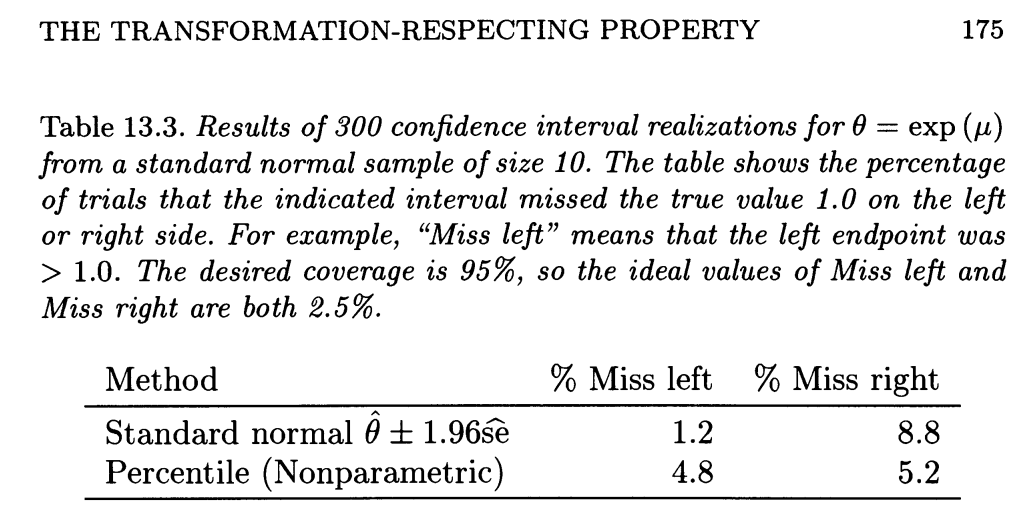
\includegraphics[width=1 \linewidth]{13/t13.6.png}}
\end{figure}

В таблице изображено процентное количество пропущеннх стандартным и процентильным интервалом значений слева и справа, для 500 смоделированных выборок. Цель не попадает в покрытие в $25 \%$ случаев для каждой стороны. Процентильный интервал обеспечивает лучший баланс между левой и правой границой, но, как и стандартный интервал, в целом он все еще не даёт достаточно хорошее покрытие. Это следствие непараметрического вывода: процентильный
интервал не знает основного нормального распределения и вместо него использует эмпирическое распределение. В этом случае он недооценивает хвост распределения $\hat{\theta}^{*}$. Более продвинутые бутстреп интервалы, подобные тем, которые будут обсуждаться в 14 и 22 главах, могут частично исправить эту неполноту покрытия.
